\subsection{Conducting and reporting the search}\label{subsec:conducting-and-reporting-the-search}

After finishing the preparations, the next step is to \textbf{perform the searches} in the engines and \textbf{document the results} (search date, search areas, number of results).
The searches were performed from February 6$^{th}$ to February 9$^{th}$, 2023.
Scopus search returned 1414 results;
Web of Science search returned 856 documents.

While performing the search, the literature was \textbf{tentatively screened for inclusion} based on titles and abstracts of works.
Papers were chosen if they:
\begin{itemize}
    \item could potentially present a representation of user interface/a UIDL,
    \item could potentially present an approach to MBUID that might use a UI representation,
    \item could potentially present a review of UI representations,
    \item could potentially discuss the problem of expressiveness of UI representations.
\end{itemize}
\textbf{The same criteria were used to look for relevant papers in the next steps.}
The screening was rather broad and not too precise, so that \textbf{as much relevant work as possible is identified};
papers unrelated to the stated problem would be discarded during later stages of the review.
This stage resulted in 133 documents found in Scopus and 77 documents found in Web of Science.
After merging the two sets and removing duplicate papers, 154 documents were left for further consideration.

In the second stage of the review, the set of papers was reviewed again in order to eliminate documents not connected to the subject of the thesis.
The judgement was additionally \textbf{based on papers' introductions and conclusions}.
The process resulted in discarding of 47 papers, mostly due to focus on problems outside the area of MBUID\@.
Other reasons for exclusion included:
\begin{itemize}
    \item papers concerning functional/declarative development of UIs,
    \item papers describing methods for generation of full applications, not focused on UIs
    \item papers based on, evaluating or comparing existing UI representations.
    \item papers without a clear definition of a UI representation
\end{itemize}

The third stage of the review eliminated further papers, based on \textbf{skimming the full text of the papers}.
In this stage, 62 papers were discarded, due to the following reasons:
\begin{itemize}
    \item papers unrelated to MBUID, focused on UI or general development,
    \item papers related to problems adjacent to the thesis problem: interaction modelling, development of a MBUID environment, techniques for UI adaptation,
    \item papers relying on other paper or an existing UI description,
    \item papers without a clear definition of a UI description (or with a definition suited for a specific use case),
    \item unavailable papers.
\end{itemize}

Exclusion \textbf{based on full-text analysis} of papers was the last screening step.
In this stage, 34 papers were excluded:
\begin{itemize}
    \item papers with an unclear, informal or very simple definition of a UI description,
    \item papers that further develop existing approaches,
    \item papers that use but do not extend an existing UI representation,
    \item papers that focus on representing the UI on an abstract level (not the concrete level, according to the CRF),
\end{itemize}

To complement the database search and find additional relevant papers, a snowballing step has been executed.
The source for this step were papers or UI representations referenced by papers from the last screening step (both selected and discarded) (backward search), as well as articles that cited the papers selected in the last step (forward search).
6 additional papers were identified in this step.

\begin{figure}
    \centering
    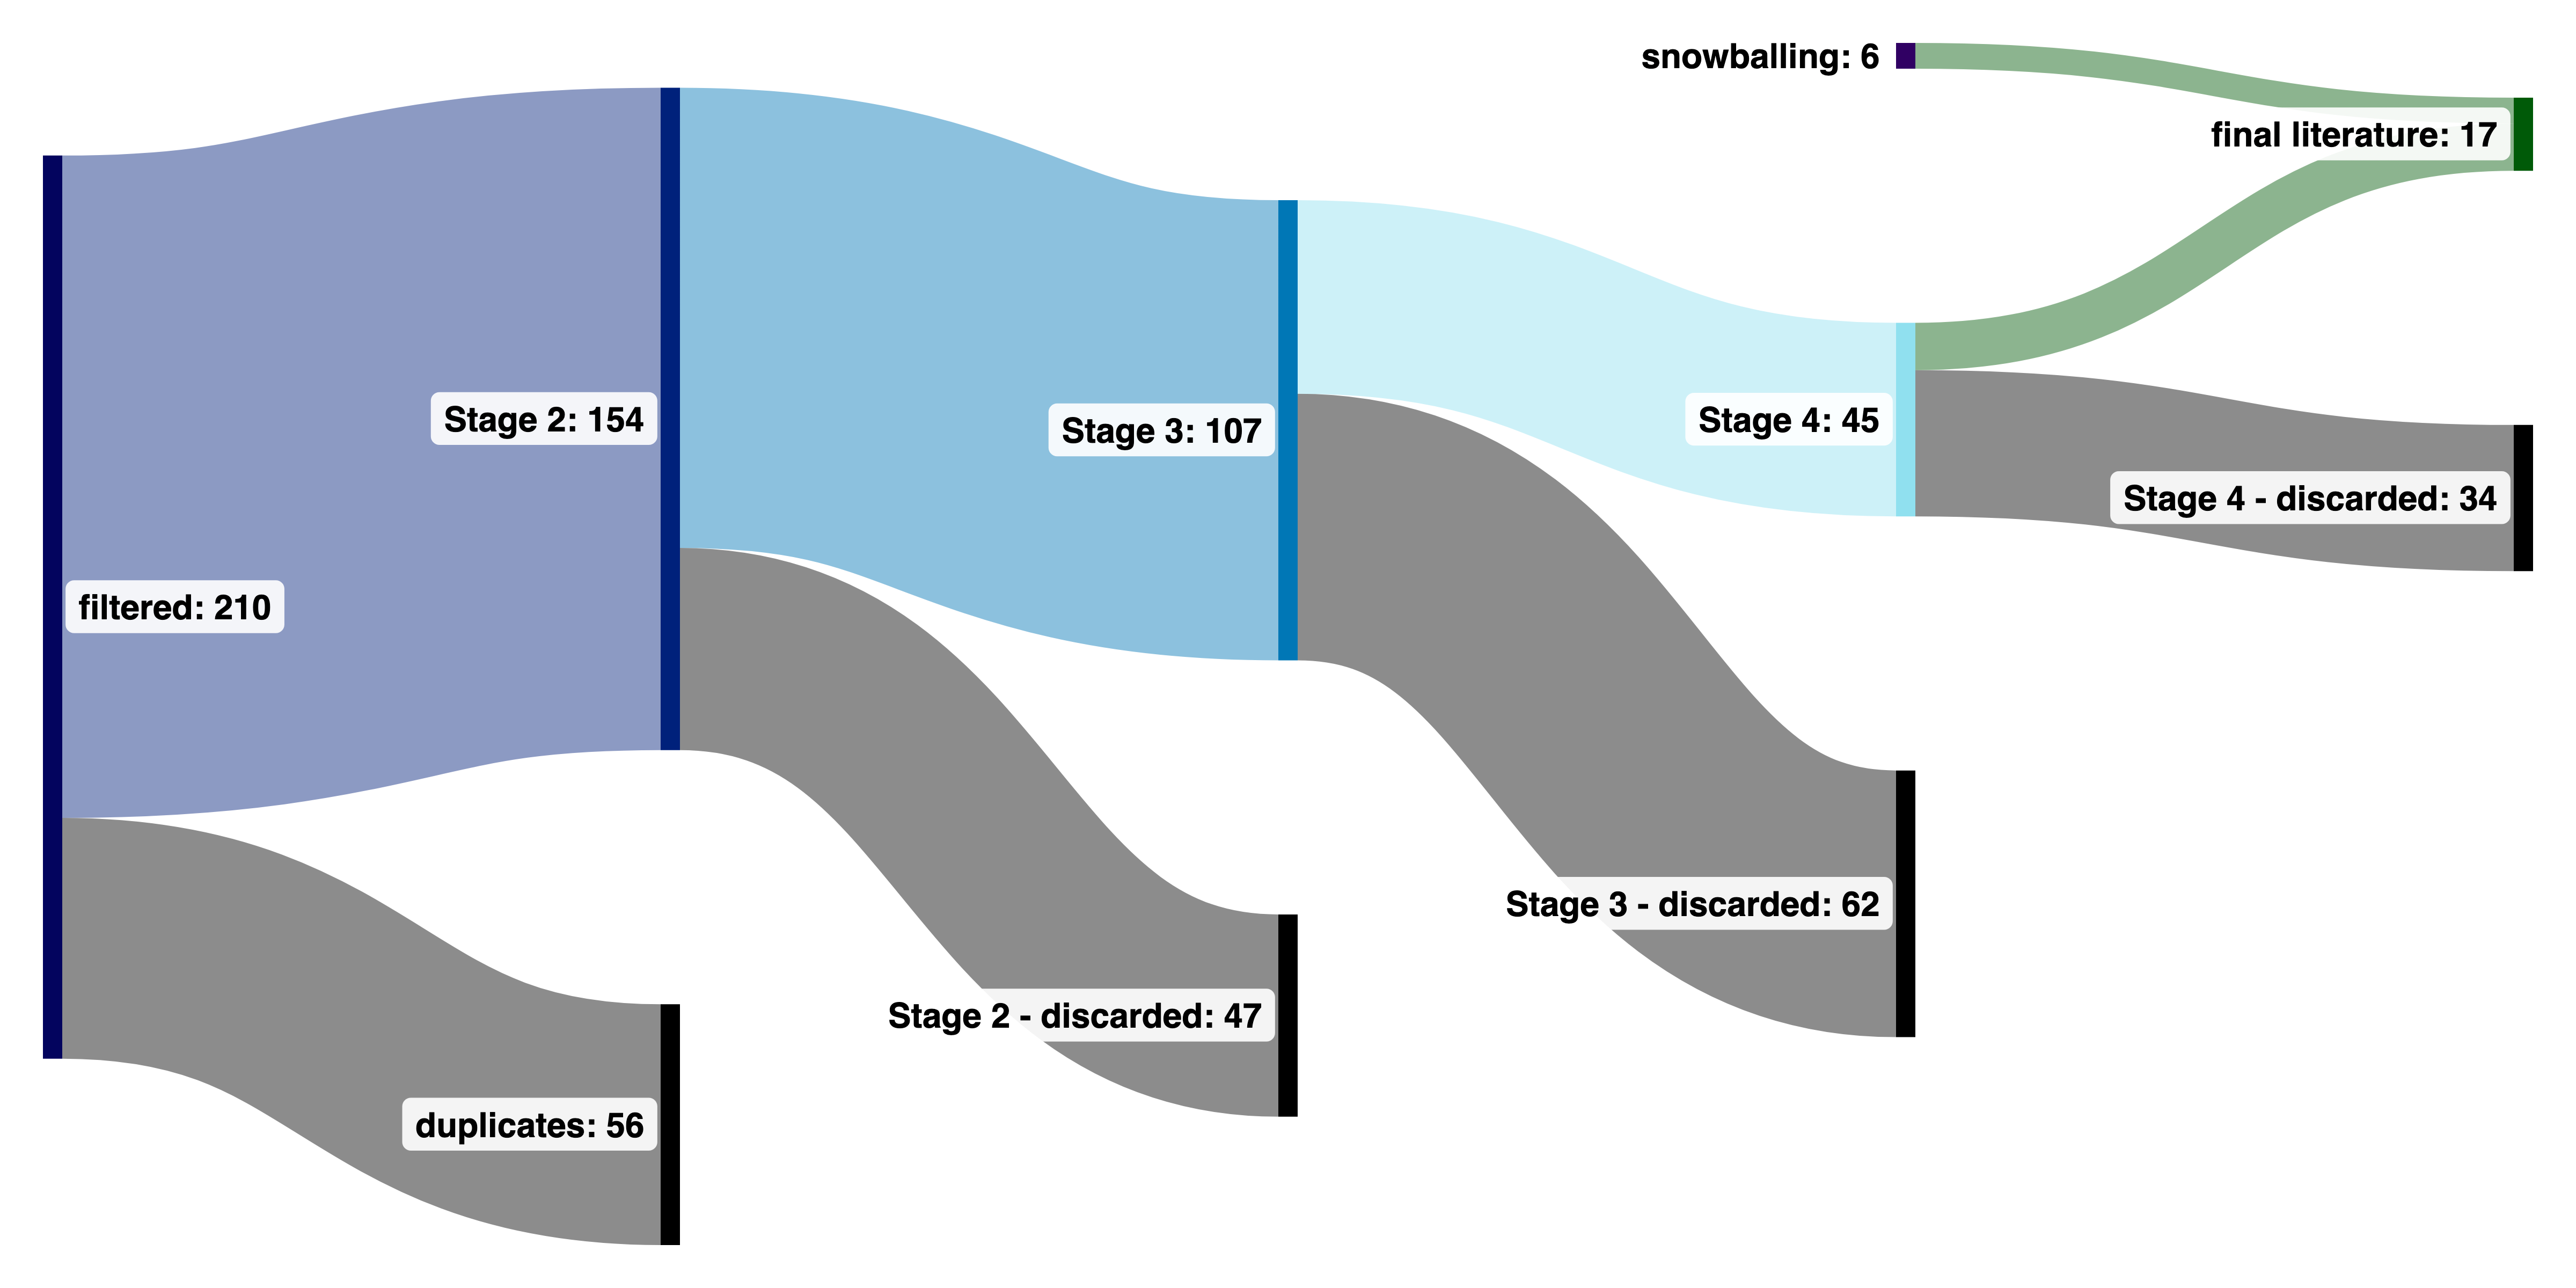
\includegraphics[width=\textwidth]{./2-literature-review/conducting-the-search}
    \caption{Visualization of subsequent steps of screening for inclusion.}
    \label{fig:conducting-the-search-vis}
\end{figure}

As a result, 17 papers were identified during the search.
The figure~\ref{fig:conducting-the-search-vis} summarizes the process.

